\begin{abstract}
	Hard parameter sharing for multi-task learning is widely used in empirical research despite the fact that its generalization properties have not been well established in many cases. This paper studies its generalization properties in a fundamental setting: How does hard parameter sharing work given multiple linear regression tasks? We develop new techniques and establish a number of new results in the high-dimensional setting, where the sample size and feature dimension increase at a fixed ratio. First, we show a sharp bias-variance decomposition of hard parameter sharing, given multiple tasks with the same features. Second, we characterize the asymptotic bias-variance limit for two tasks, even when they have arbitrarily different sample size ratios and covariate shifts. We also demonstrate that these limiting estimates for the empirical loss are incredibly accurate in moderate dimensions. Finally, we explain an intriguing phenomenon where increasing one task's sample size helps another task initially by reducing variance but hurts eventually due to increasing bias. This suggests progressively adding data for optimizing hard parameter sharing, and we validate its efficiency in text classification tasks.
\end{abstract}

\section{Introduction}\label{sec_introduction}

Hard parameter sharing (HPS) for multi-task learning is widely used in empirical research and goes back to the seminal work of \citet{C97}.
Recent work has revived interests in this approach because it improves performance and reduces the cost of collecting labeled data \cite{R17}.
It is generally applied by sharing the feature layers between all tasks while keeping an output layer for every task.
Often, hard parameter sharing offers two critical advantages if successfully applied.
First, it reduces model parameters since all tasks use the same feature space.
Second, it reduces the amount of labeled data needed from each task by augmenting the entire training dataset.

Hard parameter sharing works as an inductive transfer mechanism and a regularizer that reduces overfitting, both of which have great intuitive appeal \cite{R17}.
For example, by restricting the shared space's size, HPS encourages information sharing among multiple tasks \cite{KD12,WZR20}.
Another source of inductive bias comes from the tasks and depends on datasets' properties such as sample sizes and task covariances \cite{WZR20}.
However, how these dataset properties impact HPS has not been well established.
Part of the challenge may be that HPS' generalization performance depends intricately on the sample size ratios and covariate shifts between tasks, and is not amenable to standard concentration results.
Previous results based on Rademacher complexity or VC dimensions have considered cases where all tasks' sample sizes are equal to logarithmic factors of the feature dimension \cite{B00,MPR16}, and when all tasks' sample sizes increase simultaneously \cite{AZ05,M06}.

\begin{figure*}[!t]
	\begin{subfigure}[t]{0.5\textwidth}
		\centering
		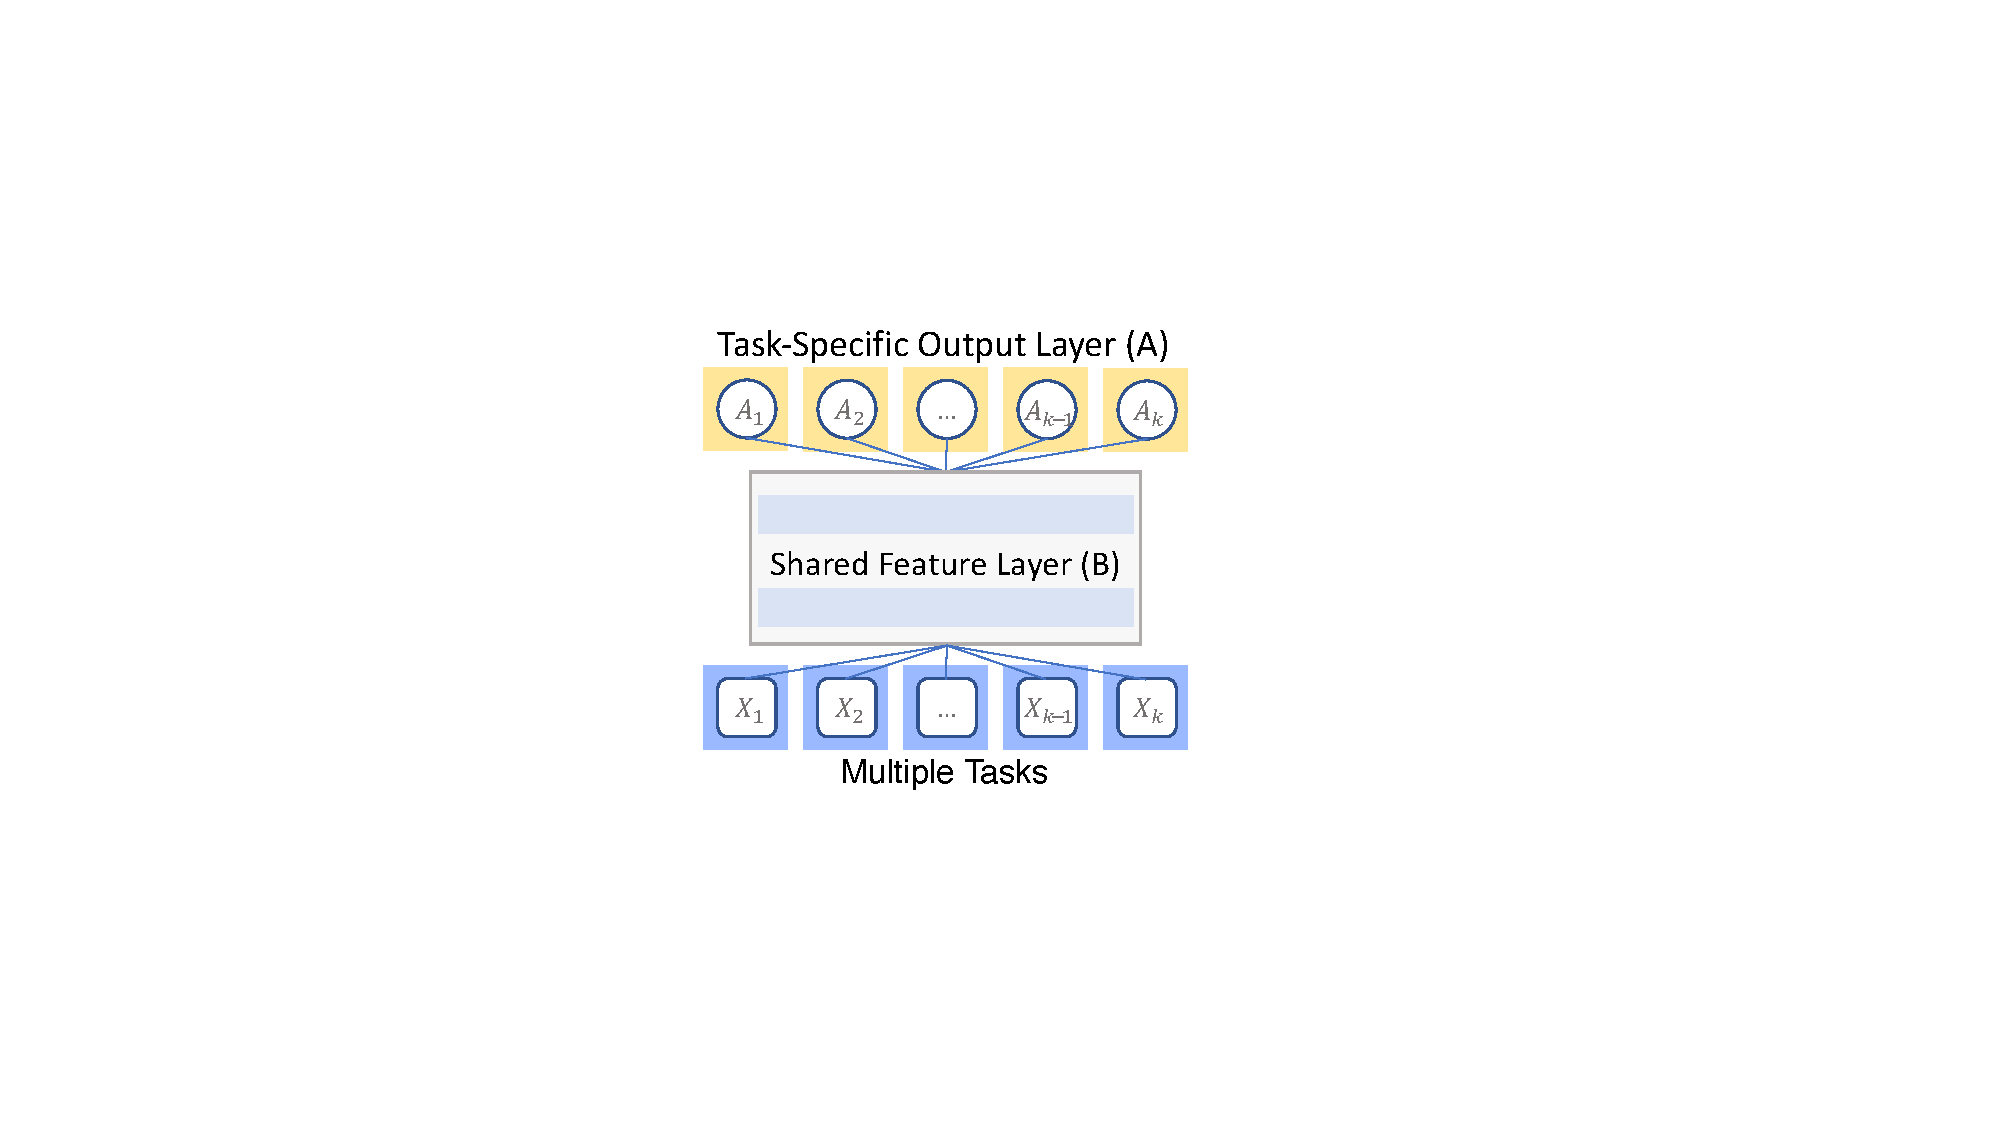
\includegraphics[width=0.45\textwidth,valign=t]{figures/mtl_model_arch.pdf}
		\caption{A hard parameter sharing architecture}
		\label{fig_intro_arch}
	\end{subfigure}\hfill
	\begin{subfigure}[t]{0.5\textwidth}
		\centering
		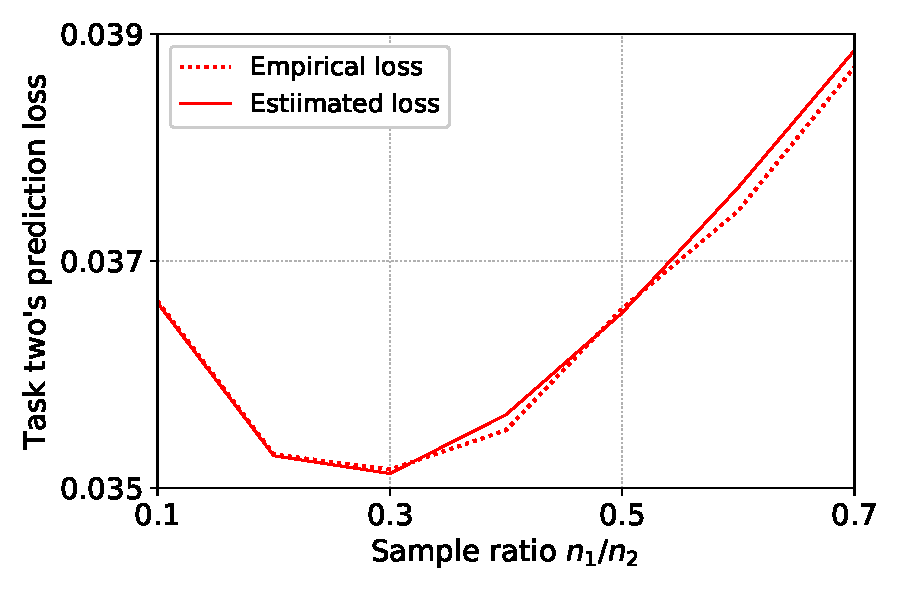
\includegraphics[width=0.745\textwidth,valign=t]{figures/sample_ratio_c2_400-eps-converted-to.pdf}
		\caption{Varying sample size ratio}
		\label{fig_intro_sample_size_b}
	\end{subfigure}
	\vspace{-0.1in}
	\caption{
	Left: an illustrative picture of HPS.
	Right: an illustrative example of using HPS for two tasks $X_1, Y_1$ and $X_2, Y_2$ with sample size $n_1, n_2$, respectively.
	Increasing $n_1/n_2$ decreases task two's prediction loss initially but increase afterward. This phenomenon occurs due to different bias-variance tradeoffs as $n_1/n_2$ increases. Our result provides an estimated loss (solid line) that accurately matches the empirical loss (dotted line).
	See Section \ref{sec_simulation} for the precise setting.}
	\label{fig_intro_sample_size}
\end{figure*}



This paper presents new techniques to study hard parameter sharing and establishes a number of new results.
We consider regression analysis, which is arguably one of the most fundamental problems in statistics and machine learning.
We are interested in the \textit{high-dimensional} setting, where each dataset's sample size and feature dimension grow linearly instead of logarithmically.
This setting captures the fact that a single task's sample size is usually insufficient for accurate learning in many applications.
For example, if a dataset's sample size is only a constant factor of dimension in linear regression, the variance is also constant (cf. Fact \ref{fact_tr}).
The high-dimensional setting is challenging but is crucial for understanding how datasets' sample sizes impact generalization performance.
